
\chapter{Methodology\label{ch:methodology}}

The idea is to extract one or more features from the 3-D information as classifiers. Together with existing classifiers found in existing work in related fields~\cite{Xu:2004tt,Yan:2007fv,Samir:2006vj}, the new features will be combined to achieve a high performance classifier for personal authentication using Support Vector Machine (SVM).

The sample data has already been collected. There are 8,000 samples from 400 different palms with both hands. Samples of a palm are collected in two separate sessions with an average interval of one month.

Experiments will be done using Matlab.

1. Extract features from each palmprint sample.

2. A subset of samples will be chosen as test set.

3. Train an authentication model based on the rest of samples.

4. Verify the samples in the test set with the trained model against their true identities.

5. Discuss the performance of the model.

%!TEX root = chapter-methodology.tex
\section{Region of Interest Extraction}
\label{sec:methodology:roiextraction}

The raw 3D palmprint image consists of 768*576 pixels with a depth value at each point. The samples are captured by a 3D palmprint acquisition device based on structured light imaging ~\cite{Zhang:2009dp}. Before any other processing, noisy pixels at the boundaries must be removed. The full resolution sample is cropped to a Region of Interest (ROI) with 400*400 resolution. A rectangle mask, from (234,68) to (634,468) is used to crop the ROI. Figure ~\ref{fig:methodology:sample-fullres} shows a full resolution sample of a palmprint and Figure ~\ref{fig:methodology:sample-roi} shows the ROI cropped. To reduce the storage and computation requirements for further processing, the ROI is down-sampled to a resolution of 200*200.

\begin{figure}[htb]
  \begin{center}
    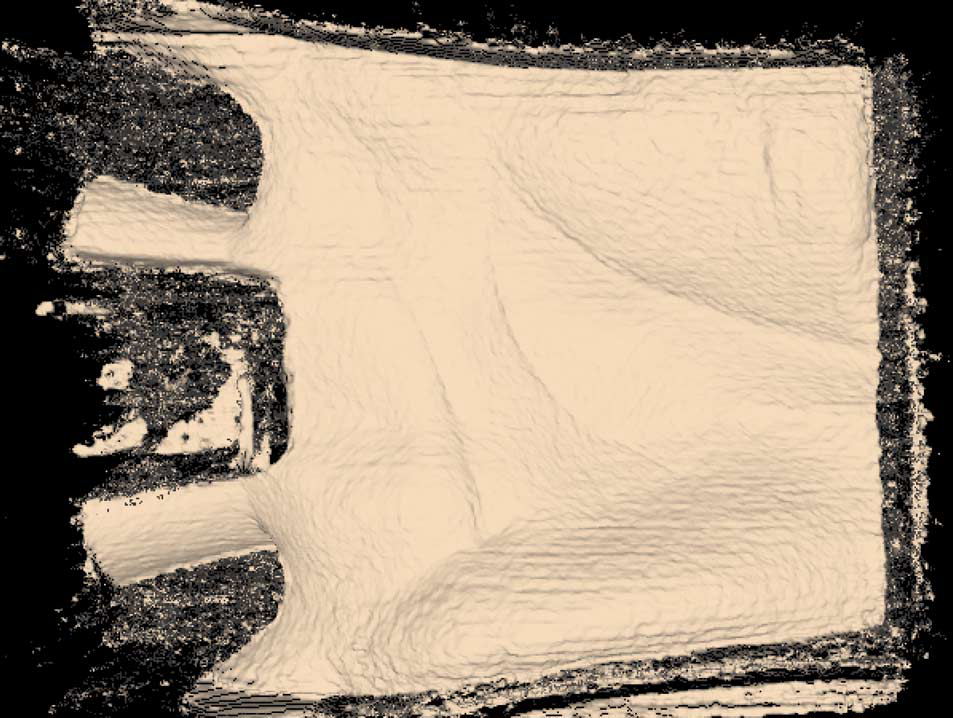
\includegraphics[width=0.9\linewidth]{ch-methodology/figures/sample-fullres}
    \caption[Full resolution 3-D palmprint sample]{Full resolution 3-D palmprint sample}    \label{fig:methodology:sample-fullres}
  \end{center}
\end{figure}

\begin{figure}[htb]
  \begin{center}
    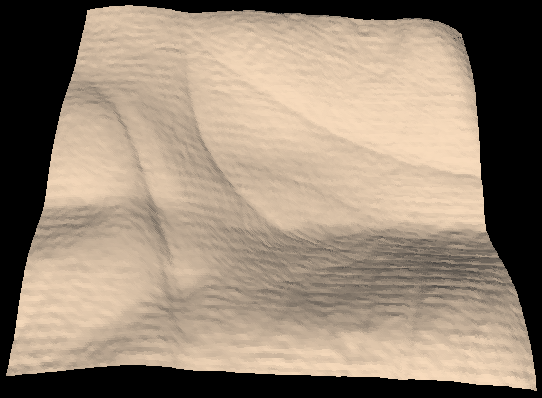
\includegraphics[width=0.9\linewidth]{ch-methodology/figures/sample-roi}
    \caption[ROI from a 3-D palmprint sample]{ROI from a 3-D palmprint sample}
    \label{fig:methodology:sample-roi}
  \end{center}
\end{figure}

The ROI data is stored in a 200 by 200 matrix,

\begin{equation}
\label{eq:methodology:roimatrix}
D=d_{ij}|i=1,2,\dots,200; j=1,2,\dots,200
\end{equation}

where $d_{ij}$ is the depth value of the $i^{th}$ row and $j^{th}$ column pixel of the ROI.

%TODO find the citation
There exists more complicated ROI extraction methods taking advantage of the 2D approaches. 2D ROI is first obtained using the algorithm in ~\cite{Zhang:2003uf}. As the 2D sample captured is pixel-to-pixel matched to the 3D sample, using the exact 2D ROI for the 3D sample is trivial.

The cropping ROI extraction approach used here is much easier and faster than the one proposed in [4]. The reason to adopt this naive approach is that the features are invariant to rotation and translation. It is unnecessary to fully align every sample. Another consideration is that when the 3D information is the only data available, it is not feasible to apply the same 2D algorithm to the depth image.

Even if the samples are cropped to the center area, it is still possible that some noisy pixels are included. If the gradient

\begin{equation}
|\nabla D|=\sqrt{
\left(\frac{\partial{D}}{\partial{x}}\right)^2 +
\left(\frac{\partial{D}}{\partial{y}}\right)^2
}
\end{equation}

is larger than a given threshold, the pixel is regarded as noisy. Another 200 by 200 matrix,

\begin{equation}
\label{eq:methodology:roimask}
M=m_{ij}|i=1,2,\dots,200;j=1,2,\dots,200
\end{equation}

is used to represent the mask, where $m_{ij}=0$ marks the noisy pixels while $m_{ij}=1$ marks the normal ones.
\section{Feature Calculation}
\label{sec:methodology:featurecalc}

Using the ROI obtained from the original 3D palmprint data, three kinds of features to describe the shape of the 3D palmprint: Maximum Depth (MD) of palm center, the Horizontal Cross-section Area (HCA) of different levels and the Radial Line Length (RLL) from the centroid to the boundary of 3D palmprint horizontal cross-section of different levels.

%!TEX root = featurecalc.tex
\subsection{Maximum Depth (MD)}
\label{ssec:methodology:md}

MD means the maximum depth value of the 3D palm from a reference plane. The reference plane is decided using a rectangle obtained by experience. The top left and bottom right pixels of the rectangle are (65,6) and (136,35). These parameters are denoted as $R_s=65, R_e=136, C_s=6$ and $C_e=35$, i.e. the starting(ending) row(column). By examine a random 20 samples, gradient of this area is relatively small.

The depth of the reference plane is defined as the mean depth of the points contained by this rectangle

\begin{equation}
d_r = {1\over{
\sum \limits_{i=R_s}^{R_e} \sum \limits_{j=C_s}^{C_e} m_{ij}
}}
\sum \limits_{i=R_s}^{R_e} \sum \limits_{j=C_s}^{C_e} (d_{ij} \cdot d_{ij})
\end{equation}

where $d_{ij}$ and $m_{ij}$ are the elements defined in ~\ref{eq:methodology:roimatrix} and ~\ref{eq:methodology:roimask}

After getting the depth of the reference plane, we find the maximum depth $d_{max}$ in another region with $R_s=41, R_e=160, C_s=65$ and $C_e=190$.

\begin{equation}
d_{max} = \max \limits_{i=R_s}^{R_e} (\max \limits_{j=C_s}^{C_e} (d_{ij}) )
\end{equation}


The Maximum Depth (MD) is then defined as

\begin{equation}
\label{eq:methodology:md}
MD= d_{max} - d_r
\end{equation}
%!TEX root = featurecalc.tex
\subsection{Horizontal Cross-section Area}
\label{ssec:methodology:hca}

When 3D ROI is examined in a contour view as shown in Figure ~\ref{fig:methodology:roicontour}, it is obvious that the regions of different given depth ranges can be used to describe a sample.

\begin{figure}[htb]
\begin{center}
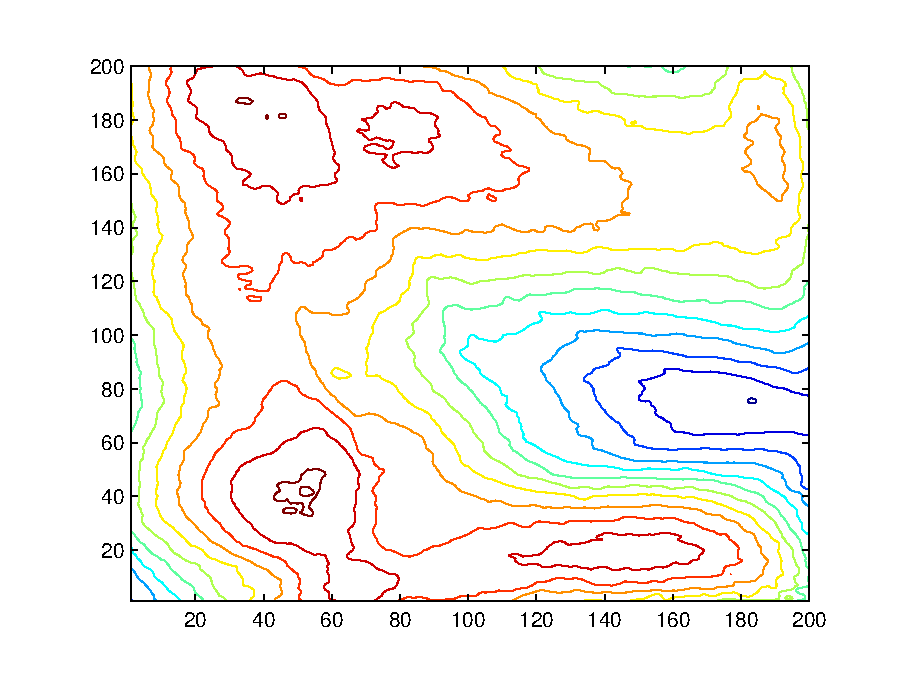
\includegraphics[width=0.9\linewidth]{ch-methodology/figures/roicontour}
\caption[Contour view of a 3D ROI]{Contour view of a 3D ROI}
\label{fig:methodology:roicontour}
\end{center}
\end{figure}

A group of equidistant horizontal planes cut the 3D ROI as shown in Figure ~\ref{fig:methodology:planecut}. Figure ~\ref{fig:methodology:roicontour} shows that most of the deeper level (enclosed with blue curves) are connected. These are more stable in response to noise or transformation.

\begin{figure}[htb]
\begin{center}
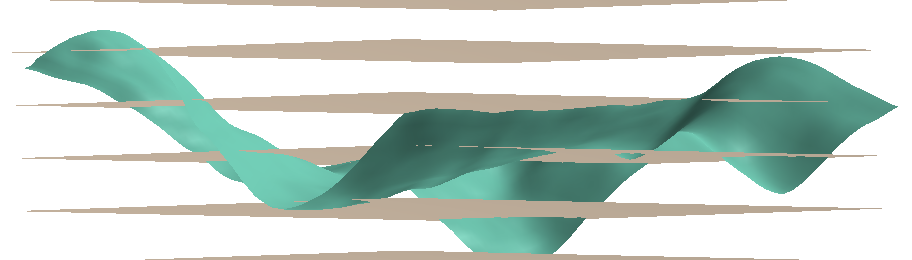
\includegraphics[width=0.9\linewidth]{ch-methodology/figures/planecut}
\caption[3D ROI cut by parallel horizontal planes]{3D ROI cut by parallel horizontal planes}
\label{fig:methodology:planecut}
\end{center}
\end{figure}


To get a stable HCA, we take into consideration only the levels from the deepest point to the reference plane, defined in Section ~\ref{ssec:methodology:md}. Suppose we divide this region into $N$ levels. Every level $G^k, k=1,2,\dots,N$ is described with a 200 by 200 matrix and calculated as

\begin{equation}
G^k_{ij} =
\begin{cases}
1 & \text{if } d_{ij}>h\cdot(N-k+1)/N,\\
0 & \text{otherwise}
\end{cases}
k=1,2,\dots,N;i=1,2,\dots,200;j=1,2,\dots,200;
\end{equation}

where $d_{ij}$ is the depth value of the $i^{th}$ row and $j^{th}$ column pixel of the ROI defined in ~\ref{eq:methodology:roimatrix} and $h$ is the palmprint depth defined by ~\ref{eq:methodology:md}.

To stabilize the areas, the growth of higher level is constrained to its previous level except the first level. That is

\begin{equation}
L^k=
\begin{cases}
G^1                             & k=1 \\
G^k \cap (L^{k-1} \oplus \Theta^{k-1}) & k=2,3,\dots,N
\end{cases}
\end{equation}

where $\cap$ denotes logical AND, $\oplus$ denotes a morphological dilation operation and  $\Theta^{k}$ is a disk morphological structuring element whose size can be calculated by $35-3 \times k$ (which is suitable for N = 8 by experience).

\begin{figure}[htb]
\begin{center}
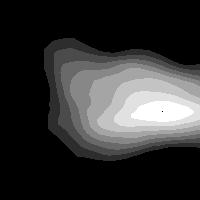
\includegraphics[width=0.9\linewidth]{ch-methodology/figures/hcastack}
\caption[$L^k$ shown stacked when $N=8$]{$L^k$ shown stacked when $N=8$}
\label{fig:methodology:hcastack}
\end{center}
\end{figure}

Figure ~\ref{fig:methodology:hcastack} shows an example of all the levels stacked together.

\begin{figure}[htb]
\centering
\subfigure[$k=1$]{
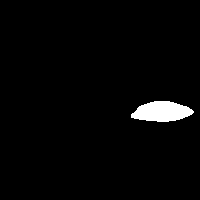
\includegraphics[height=0.18\textheight]{ch-methodology/figures/hca1-1}
\label{fig:methodology:hcalevels:1-1}
}\hspace{0.15\linewidth}
\subfigure[$k=2$]{

\includegraphics[height=0.18\textheight]{ch-methodology/figures/hca1-2}
\label{fig:methodology:hcalevels:1-2}
}\\
\subfigure[$k=3$]{
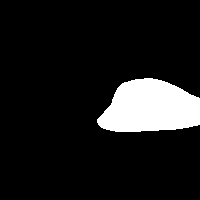
\includegraphics[height=0.18\textheight]{ch-methodology/figures/hca1-3}
\label{fig:methodology:hcalevels:1-3}
}\hspace{0.15\linewidth}
\subfigure[$k=4$]{
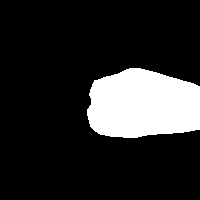
\includegraphics[height=0.18\textheight]{ch-methodology/figures/hca1-4}
\label{fig:methodology:hcalevels:1-4}
}\\
\subfigure[$k=5$]{
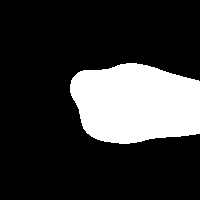
\includegraphics[height=0.18\textheight]{ch-methodology/figures/hca1-5}
\label{fig:methodology:hcalevels:1-5}
}\hspace{0.15\linewidth}
\subfigure[$k=6$]{
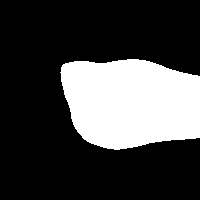
\includegraphics[height=0.18\textheight]{ch-methodology/figures/hca1-6}
\label{fig:methodology:hcalevels:1-6}
}\\
\subfigure[$k=7$]{
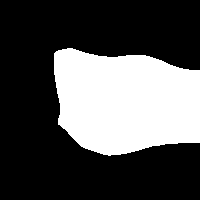
\includegraphics[height=0.18\textheight]{ch-methodology/figures/hca1-7}
\label{fig:methodology:hcalevels:1-7}
}\hspace{0.15\linewidth}
\subfigure[$k=8$]{
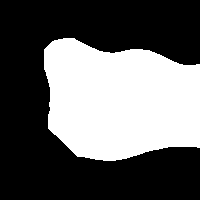
\includegraphics[height=0.18\textheight]{ch-methodology/figures/hca1-8}
\label{fig:methodology:hcalevels:1-8}
}
\caption[$L^k$ of one sample from palm 1]{$L^k$ for $k=1,2,\dots,8$ of a 3D ROI from a palmprint sample}
\label{fig:methodology:hcalevels1}
\end{figure}


\begin{figure}[htb]
\centering
\subfigure[$k=1$]{
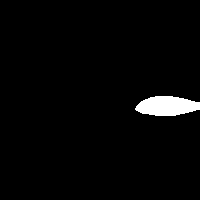
\includegraphics[height=0.18\textheight]{ch-methodology/figures/hca2-1}
}\hspace{0.15\linewidth}
\subfigure[$k=2$]{
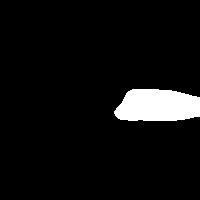
\includegraphics[height=0.18\textheight]{ch-methodology/figures/hca2-2}
}\\
\subfigure[$k=3$]{
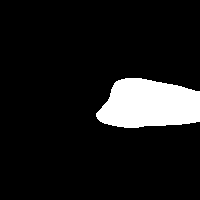
\includegraphics[height=0.18\textheight]{ch-methodology/figures/hca2-3}
}\hspace{0.15\linewidth}
\subfigure[$k=4$]{
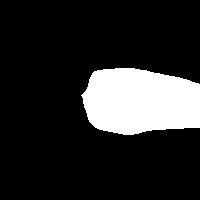
\includegraphics[height=0.18\textheight]{ch-methodology/figures/hca2-4}
}\\
\subfigure[$k=5$]{
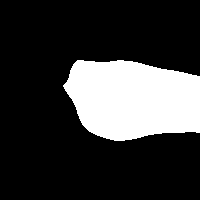
\includegraphics[height=0.18\textheight]{ch-methodology/figures/hca2-5}
}\hspace{0.15\linewidth}
\subfigure[$k=6$]{
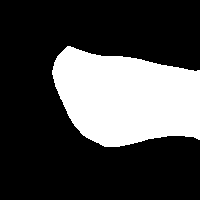
\includegraphics[height=0.18\textheight]{ch-methodology/figures/hca2-6}
}\\
\subfigure[$k=7$]{
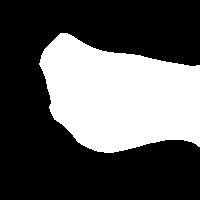
\includegraphics[height=0.18\textheight]{ch-methodology/figures/hca2-7}
}\hspace{0.15\linewidth}
\subfigure[$k=8$]{
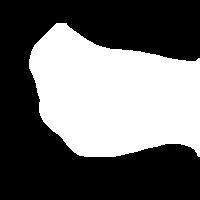
\includegraphics[height=0.18\textheight]{ch-methodology/figures/hca2-8}
}
\caption[$L^k$ of another sample from palm 1]{$L^k$ for $k=1,2,\dots,8$ of a 3D ROI from another palmprint sample from the same person as in Figure ~\ref{fig:methodology:hcalevels1}}
\label{fig:methodology:hcalevels2}
\end{figure}

\begin{figure}[htb]
\centering
\subfigure[$k=1$]{

\includegraphics[height=0.18\textheight]{ch-methodology/figures/hca3-1}
}\hspace{0.15\linewidth}
\subfigure[$k=2$]{

\includegraphics[height=0.18\textheight]{ch-methodology/figures/hca3-2}
}\\
\subfigure[$k=3$]{

\includegraphics[height=0.18\textheight]{ch-methodology/figures/hca3-3}
}\hspace{0.15\linewidth}
\subfigure[$k=4$]{
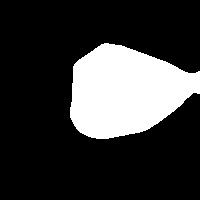
\includegraphics[height=0.18\textheight]{ch-methodology/figures/hca3-4}
}\\
\subfigure[$k=5$]{
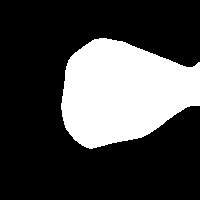
\includegraphics[height=0.18\textheight]{ch-methodology/figures/hca3-5}
}\hspace{0.15\linewidth}
\subfigure[$k=6$]{
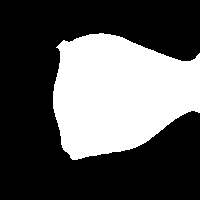
\includegraphics[height=0.18\textheight]{ch-methodology/figures/hca3-6}
}\\
\subfigure[$k=7$]{
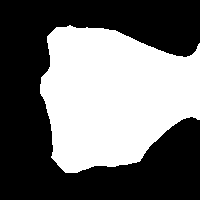
\includegraphics[height=0.18\textheight]{ch-methodology/figures/hca3-7}
}\hspace{0.15\linewidth}
\subfigure[$k=8$]{
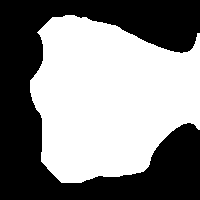
\includegraphics[height=0.18\textheight]{ch-methodology/figures/hca3-8}
}
\caption[$L^k$ of one sample from palm 2]{$L^k$ for $k=1,2,\dots,8$ of a 3D ROI from a palmprint sample from the a different person from that of Figure ~\ref{fig:methodology:hcalevels1}}
\label{fig:methodology:hcalevels3}
\end{figure}

\begin{figure}[htb]
\centering
\subfigure[$k=1$]{

\includegraphics[height=0.18\textheight]{ch-methodology/figures/hca4-1}
}\hspace{0.15\linewidth}
\subfigure[$k=2$]{

\includegraphics[height=0.18\textheight]{ch-methodology/figures/hca4-2}
}\\
\subfigure[$k=3$]{
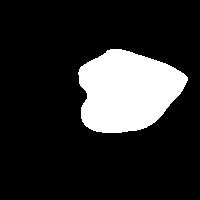
\includegraphics[height=0.18\textheight]{ch-methodology/figures/hca4-3}
}\hspace{0.15\linewidth}
\subfigure[$k=4$]{
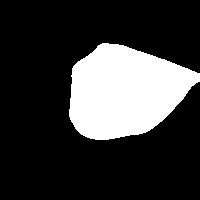
\includegraphics[height=0.18\textheight]{ch-methodology/figures/hca4-4}
}\\
\subfigure[$k=5$]{
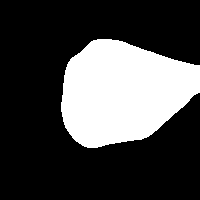
\includegraphics[height=0.18\textheight]{ch-methodology/figures/hca4-5}
}\hspace{0.15\linewidth}
\subfigure[$k=6$]{
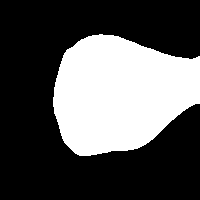
\includegraphics[height=0.18\textheight]{ch-methodology/figures/hca4-6}
}\\
\subfigure[$k=7$]{
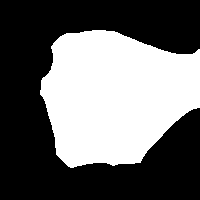
\includegraphics[height=0.18\textheight]{ch-methodology/figures/hca4-7}
}\hspace{0.15\linewidth}
\subfigure[$k=8$]{
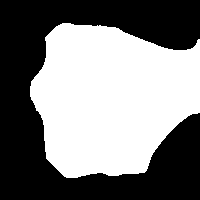
\includegraphics[height=0.18\textheight]{ch-methodology/figures/hca4-8}
}
\caption[$L^k$ of another sample from palm 2]{$L^k$ for $k=1,2,\dots,8$ of a 3D ROI from another palmprint sample from the same person as in Figure ~\ref{fig:methodology:hcalevels3}}
\label{fig:methodology:hcalevels4}
\end{figure}

Figure ~\ref{fig:methodology:hcalevels1} and ~\ref{fig:methodology:hcalevels2} shows the cross-sectional area feature from two samples collected from one palm. Figure ~\ref{fig:methodology:hcalevels3} and ~\ref{fig:methodology:hcalevels4} are extracted from two samples from another palm.

\subsection{Radial Line Length (RLL)}
\label{ssec:methodology:rll}

HCA is a coarse summary of the ROI characteristics. Different sample may have a similar area but dramatically different shape or contour of that area. To describe this shape characteristic, we need more elements to represent the ROI. The Radial Line Length (RLL) is then introduced for this purpose.

First, we calculate the centroid of the first level  $L^1$, thereafter we treat it as the reference point $P_{ref}$ for all levels. Then, from $P_{ref}$ we draw M radial lines which intersect with the contour of every level. RLL is defined as the distance from the intersection point to $P_{ref}$. The radial lines are distributed at equal angles. We record these radial lines from the inner layers to the outer layers starting with the horizontal direction by an $M$ by $N$ dimensional vector
\begin{equation}
R_i, i=1,2,\dots,M\times N
\end{equation}
where $M$ is the number of radial lines and $N$ is the number of cross-sections.

Figure ~\ref{fig:methodology:rll8} through ~\ref{fig:methodology:rll64} show some examples of RLL. This is a more detailed description than HCA as it takes the shape of each area into consideration.

\begin{figure}[htb]
  \begin{center}
    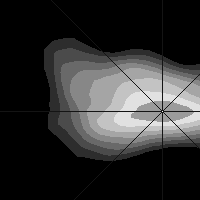
\includegraphics[width=0.4\linewidth]{ch-methodology/figures/rll8}
    \caption[8 radial lines starting from the reference point]{8 radial lines starting from the reference point}
    \label{fig:methodology:rll8}
  \end{center}
\end{figure}

\begin{figure}[htb]
  \begin{center}
    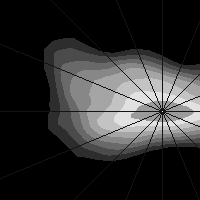
\includegraphics[width=0.4\linewidth]{ch-methodology/figures/rll16}
    \caption[16 radial lines starting from the reference point]{16 radial lines starting from the reference point}
    \label{fig:methodology:rll16}
  \end{center}
\end{figure}

\begin{figure}[htb]
  \begin{center}
    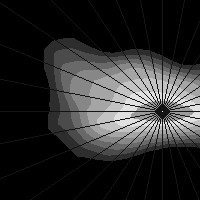
\includegraphics[width=0.4\linewidth]{ch-methodology/figures/rll32}
    \caption[32 radial lines starting from the reference point]{32 radial lines starting from the reference point}
    \label{fig:methodology:rll32}
  \end{center}
\end{figure}

\begin{figure}[htb]
  \begin{center}
    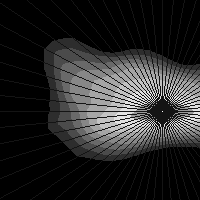
\includegraphics[width=0.4\linewidth]{ch-methodology/figures/rll64}
    \caption[64 radial lines starting from the reference point]{64 radial lines starting from the reference point}
    \label{fig:methodology:rll64}
  \end{center}
\end{figure}



The above three features are mainly determined by the central region of the palm. This region is certainly contained by the ROI described in Section ~\ref{sec:methodology:roiextraction} which makes these features insensitive to translation and rotation. Although the RLL feature can be affected by rotation as the contours change smoothly, if the rotation is small then the variation of the RLL feature will also be small. Actually, there are some restricting pegs on the capture device which can guide the users to put their hands on the proper place as described in ~\cite{Zhang:2009dp}. Furthermore, we assume the user is cooperative when collecting data as we aim at civil rather than law enforcement applications.

%!TEX root = chapter-methodology.tex
\section{Feature Matching}
\label{sec:methodology:featurematch}

%TODO find the citaions
The classification of biometrics speeds up the identification process by reducing the number of comparisons that must be made. There are two kinds of classification techniques: exclusive classification and continuous classification. Both fingerprint ~\cite{Henry:1900vc} and palmprint classifications ~\cite{Wu:2004kx} make use of exclusive classification. The main problem of this technique is that it uses only a small number of classes and the samples are unevenly distributed between them, with more than 90\% of the samples being in just two or three classes. A further problem with exclusive classification is that when classification is performed automatically, it is necessary to handle errors and rejected samples gracefully, which is a hard problem in practice. In contrast, for continuous classification, samples are not partitioned into disjoint classes but rather associated with numerical vectors which represent features of the samples. These feature vectors are created through a similarity-preserving transformation so that similar samples are mapped into close points in the multi-dimensional space ~\cite{Maltoni:wn}. The continuous classification technique is adopted. As the features combining MD, HCA and RLL are high-dimensional, LDA is used for dimension reduction. Coarse-level matching and Ranking Support Vector Machine (RSVM) are applied to the low dimensional vectors for efficient palmprint recognition.

\subsection{Dimension Reduction}
\label{ssec:methodology:lda}

LDA is a state-of-the-art dimensionality reduction technique widely used in classification problems. The objective is to find the optimal projection which simultaneously minimizes the within-class distance and maximizes the between-class distance, thus achieving maximum discrimination (Here, the “class” is used to denote the identity of the subjects, e.g. the samples collected from one palm are regarded as one class). However, the traditional LDA requires the within-class scatter matrix to be nonsingular, which means the sample size should be large enough compared with its dimension, but is not always possible. In this paper, we therefore adopt the orthogonal LDA (OLDA) proposed in [17], where the vectors of the optimal projection are calculated using the training database and the optimal projecting vectors are orthogonal to each other.
Suppose the 3D ROI has been divided to N levels and that M radial lines are used to represent the level contours. We can list the global features as a column vector,  , with   rows. Given a training database which has n samples and k classes as  , where   and  , adopting OLDA [17] the optimal projection W can be calculated as follows.
First, the within-class scatter matrix  , the between-class scatter matrix   and total scatter matrix   can be expressed as
                              (6)
where
                           (7)
                         (8)
                                         (9)
where   is the centroid of the ith class  ,   is the centroid of all the training samples ,   and  .
After calculating  ,   and  , the reduced Singular Value Decomposition (SVD) is applied to  .
                                     (10)
Denote   and compute the SVD of B.
                                          (11)
Let
                                              (12)
                                              (13)
and denote   the first   columns of the matrix D. Then, compute the QR decomposition of  .
                                    (14)
where Q is the desired orthogonal matrix and optimal projection, i.e.  .
After getting the optimal projection W, we can map the   dimensional vector F to a lower dimensional space
                                             (15)
where   is a   dimensional vector with  .

%!TEX root = featurematch.tex
\subsection{Coarse-level Matching}
\label{ssec:methodology:naive}

For palmprint recognition, we need a measurement of similarity between two samples. If the similarity is high, we have a high confidence to believe that the two samples are from the same person. Otherwise we reject to claim that.

After mapping the high-dimensional feature vector to $\Gamma$-dimensional vector $\tilde{F}$, the similarity between two samples can be calculated as

\begin{equation}
Similarity= \| \tilde{F}_1 -\tilde{F}_2 \|
= \sum \limits_{i=1}^{\Gamma} (f_i^1-f_i^2)^2
\label{eq:methodology:similarity}
\end{equation}

\begin{figure}[htb]
  \begin{center}
    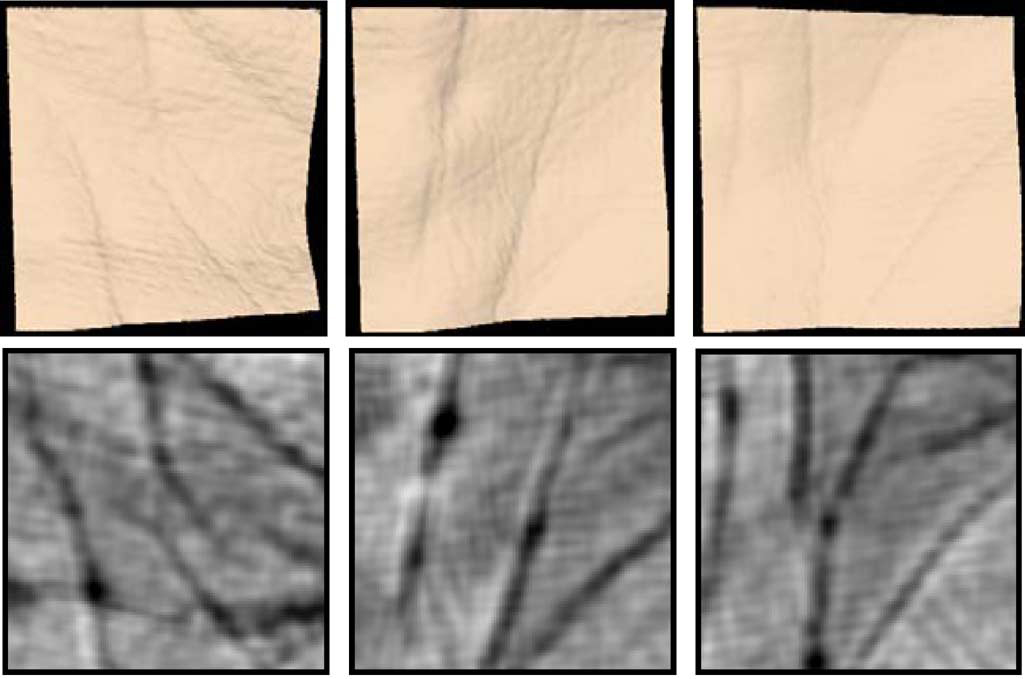
\includegraphics[width=0.9\linewidth]{ch-methodology/figures/mci1}
    \caption[MCI for ROIs from different palms]{Mean Curvature Image for ROIs from three different palms}    \label{fig:methodology:mci1}
  \end{center}
\end{figure}

\begin{figure}[htb]
  \begin{center}
    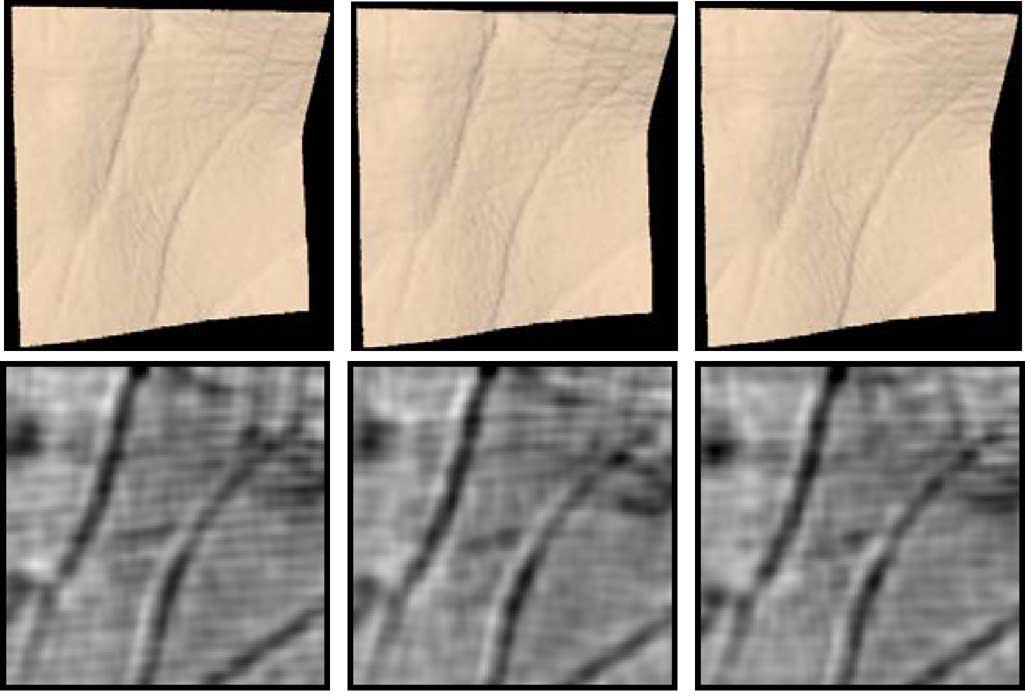
\includegraphics[width=0.9\linewidth]{ch-methodology/figures/mci2}
    \caption[MCI for ROIs from the same palm]{Mean Curvature Image for ROIs from three samples of the same palm}    \label{fig:methodology:mci2}
  \end{center}
\end{figure}

There are other features extracted from the same dataset such as Mean Curvature Image in ~\cite{Zhang:2009dp}. Figure ~\ref{fig:methodology:mci1} shows the ROI and MCI extracted from three different palms while Figure ~\ref{fig:methodology:mci2} show samples from the same palm. The corresponding matching score is defined as

\begin{equation}
Y=\frac{
    2\sum \limits_{i=1}^{n} \sum \limits_{j=1}^{m} Z_d(i,j) \cap Z_t(i,j)
}
{
    \sum \limits_{i=1}^{n} \sum \limits_{j=1}^{m} Z_d(i,j) +
    \sum \limits_{i=1}^{n} \sum \limits_{j=1}^{m} Z_t(i,j)
}
\end{equation}

where symbol $\cap$ represents the logical AND operation, $Z_d$ and $Z_t$ are two binarized MCIs. Due to the fact that MCI is covariant to shifting, the actual matching process for MCI is repeated by shifting the image with 4 different displacement in 8 directions. A total of 33 matching scores are calculated and the maximum is adopted as the overall matching score.

Although MCI feature is more descriptive, it takes up more storage ($200\times200$ floats to store the feature image). Compared to the computation in ~\ref{eq:methodology:similarity}, the MCI matching process requires far more computation and is therefore significantly slower.
% Table generated by Excel2LaTeX from sheet 'Sheet1'
\begin{table}[htbp]
  \centering
  \caption{Penetration rate and error rate using RSVM}
    \begin{tabular}{|c|c|}
    \hline
    Penetration rate (\%) & Error rate (\%) \\
    \hline
    30    & 1.3 \\ \hline
    27.5  & 1.33 \\ \hline
    25    & 1.37 \\ \hline
    22.5  & 1.42 \\ \hline
    20    & 1.49 \\ \hline
    17.5  & 1.63 \\ \hline
    15    & 1.87 \\ \hline
    12.5  & 2.48 \\ \hline
    10    & 3.35 \\ \hline
    7.5   & 4.41 \\ \hline
    5     & 5.88 \\
    \hline
    \end{tabular}%
  \label{tab:experiment:svm}%
\end{table}%


